\documentclass[11pt]{article}
\usepackage[margin=1in]{geometry}
\usepackage{amsmath,amssymb}
\usepackage{graphicx}
\usepackage{float}
\usepackage{hyperref}

\begin{document}

%======================================================================
\section{Does contrastive decoding correct where the hallucination is,
over the course of generation?}
%======================================================================

\paragraph{Context.}
Contrastive decoding (CD) tries to cut down hallucination by running a second,
weaker branch on a corrupted image and subtracting its distribution from the
expert's at every decoding step. In captioning this happens at every token, and the
thing it is supposed to catch keeps moving as the sentence grows. So the natural
question is a temporal one. As the caption gets longer, does CD keep pushing where
the risk actually is? The short answer is no. In two lines of algebra and one plot
we can see that the size of CD's push at each step is set by the KL between the two
branches, that this KL falls off as the caption grows, and so CD pushes hardest at
the very start, where there is almost nothing to fix, and has gone quiet by the time
the late, image-dependent words show up.

\paragraph{The mechanism, in one connection.}
Say the expert sees the clean image $x$ and the amateur sees the corrupted image
$x'$, both reading off the same generated prefix $y_{<t}$. Write the per-token gap
between them as $\Delta_t(y)=\operatorname{logit}_A(y\mid x',y_{<t})-
\operatorname{logit}_E(y\mid x,y_{<t})$. CD's logit is $z^{CD}=(1{+}\alpha)z^{E}-
\alpha z^{A}=z^{E}-\alpha\,\Delta_t$, so its correction at step $t$ is just
$-\alpha\,\Delta_t$. Now call the per-step KL between the branches the perturbation
sensitivity, $\mathrm{PS}(t)=\mathrm{KL}[p_E(\cdot\mid x,y_{<t})\,\Vert\,p_A(\cdot
\mid x',y_{<t})]$. The amateur is just the expert with its logits tilted by the
shift, $p_A\propto p_E\,e^{\Delta_t}$, and the KL of a tilt has a closed form
(Appendix~\ref{app:kl}), whose leading term is a variance:
\begin{equation}
\mathrm{PS}(t)=\psi_t(\Delta_t)-\mathbb{E}_{p_E}[\Delta_t]
             =\tfrac12\operatorname{Var}_{p_E}[\Delta_t]+O(\Delta_t^3),
\qquad \psi_t(\Delta)=\log\mathbb{E}_{p_E}\big[e^{\Delta}\big].
\label{eq:kl}
\end{equation}
So $\mathrm{PS}(t)$ is a squared (Fisher) measure of the perturbation size. CD's
correction is the shift itself, with magnitude linear in $\Delta_t$, so
\begin{equation}
\big\lVert\text{CD correction at }t\big\rVert
   =\alpha\lVert\Delta_t\rVert \;\propto\; \sqrt{\mathrm{PS}(t)}.
\label{eq:prop}
\end{equation}
The KL curve and CD's correction schedule are therefore the same curve up to a
square root. Turning $\alpha$ up or down only scales it, it never changes the shape.

\paragraph{Why the KL falls off, and why that is the wrong way round.}
Both branches use the same language weights. The only difference between them is the
image. As the sentence gets longer, the words already written drive both branches'
next-token logits in the same way and hold them together, so the one thing CD feeds
on, their disagreement about the image, keeps shrinking toward a floor. Writing the
shrinking shift as $\Delta_t\approx\Delta_0\,g(t)$ with $g$ heading down, Eq.
\eqref{eq:kl} gives $\mathrm{PS}(t)\approx\mathrm{PS}(0)\,g(t)^2$ and, by Eq.
\eqref{eq:prop}, a correction magnitude falling as $g(t)$. Hallucination risk does
not behave like this. It follows how much the image still matters, and that fades
much more slowly, since the picture stays relevant for the whole caption. So CD's
push is loaded onto the front of the sentence while the risk sits at the back, and
the two end up pulling in opposite directions in time. The picture to keep in mind:
two people describe the same photo, one sees it sharp and one sees it blurred. On
the first word they disagree a lot, because the blur is all that separates them. But
once the sentence is rolling, both are mostly just finishing it off from the words
already on the page, and the shared text pulls them back together. CD only acts
where they disagree, so its push dies away right as the late, detail-heavy words,
the ones most likely to be hallucinated, are being written.

\paragraph{Methodology.}
The whole argument leans on one empirical claim, that $\mathrm{PS}(t)$ falls with
$t$, so we check it directly. For each prompt we run CD to get a caption, and at
every generated position $t$ we grab the expert distribution $p_E(\cdot\mid x,
y_{<t})$ and the amateur distribution $p_A(\cdot\mid x',y_{<t})$ over the same
prefix, so both branches read exactly the same words and only the image input
differs, and we take $\mathrm{PS}(t)=\mathrm{KL}[p_E\Vert p_A]$. We average this
over prompts at matching positions on VisIT-Bench ($N=578$) with LLaVA-1.5-7B, for
three CD variants that differ only in how the amateur is built: VCD (a
diffusion-noised image), SID (an information-degraded view), and ICD (a text-side
instruction perturbation).

\paragraph{Results.}
All three variants tell the same story (Figure~\ref{fig:kld}). The per-step KL
climbs for a handful of tokens, then falls off monotonically and settles onto a
positive floor, which is exactly the $\mathrm{PS}(t)=\mathrm{PS}(0)\,g(t)^2$ shape.
VCD and SID each drop by about a factor of ten down the log axis. ICD sits a full
order of magnitude lower and stays almost flat, so by Eq.~\eqref{eq:prop} it is
barely correcting anything at any step. In every case the early tokens is where KLD
between amateur and expert is increasing(Exactly as predicted) and decreases as
tokens increase. Read
through Eq.~\eqref{eq:prop}, that is the temporal version of CD's miscalibration in
generation: the push is biggest at the start of the caption, where the model is
committing to ordinary syntactic, high-prior words at low risk, and has faded to
its floor by the tail, where the late object and attribute words carry the image
dependence that hallucination actually rides on.
\begin{figure}[H]
  \centering
  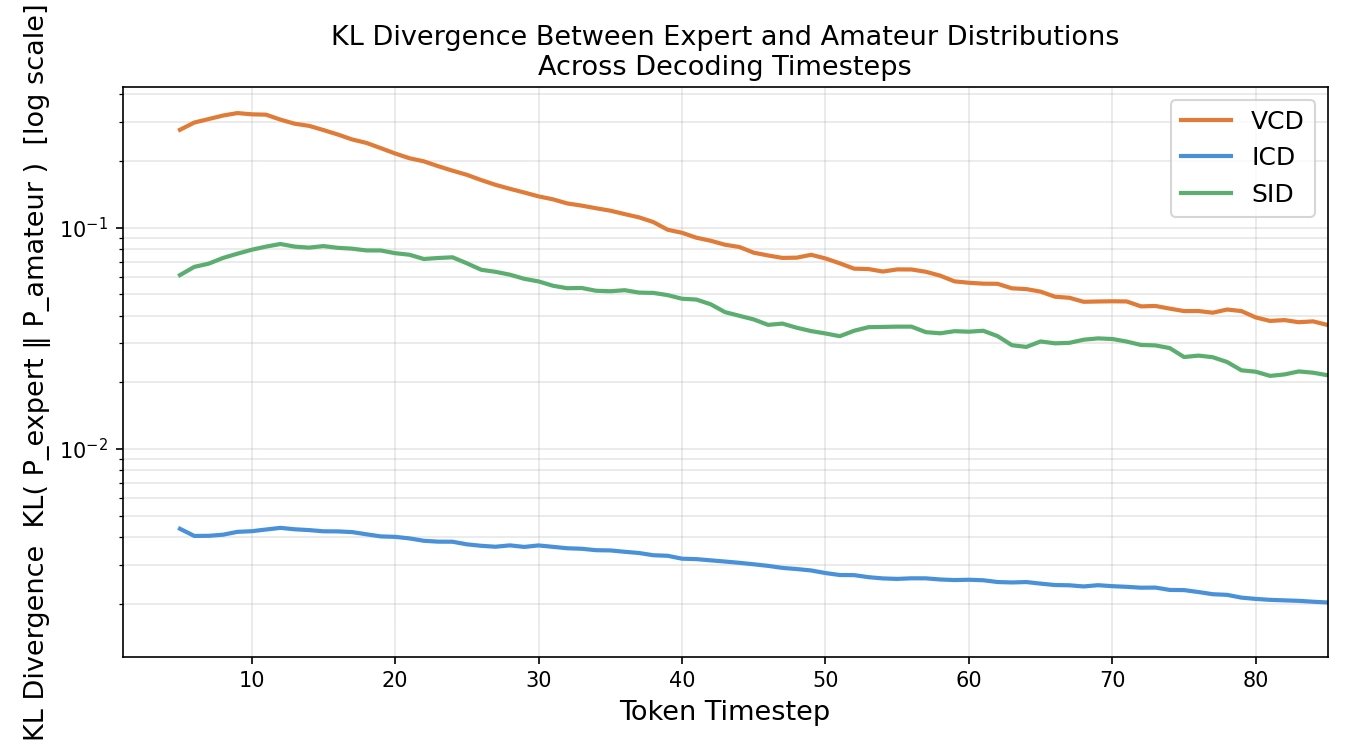
\includegraphics[width=0.82\linewidth]{kld_plot.png}
  \caption{Per-step KL between expert and amateur, $\mathrm{PS}(t)$, against token
  position on VisIT-Bench ($N=578$), log scale, for three CD variants. All fall off
  monotonically after a short early rise and level out on a positive floor. VCD and
  SID drop by roughly a factor of ten; ICD sits an order of magnitude lower and
  stays nearly flat. By Eq.~\eqref{eq:prop} the correction size tracks the square
  root of these curves, so it too is spent on the early tokens and sitting near its
  floor by the tail, which is the opposite of where hallucination risk lives.}
  \label{fig:kld}
\end{figure}

\appendix
\section{The KL of a logit tilt}
\label{app:kl}

Since $z^A=z^E+\Delta_t$, the amateur is an exponential tilt of the expert,
\begin{equation}
p_A(y)=\frac{p_E(y)\,e^{\Delta_t(y)}}{\mathbb{E}_{p_E}[e^{\Delta_t}]},
\qquad
\psi_t(\Delta)=\log\mathbb{E}_{p_E}\big[e^{\Delta}\big],
\end{equation}
so the normalizer is the log-partition (cumulant generating) function $\psi_t$. The
KL of a tilt is then exact,
\begin{equation}
\mathrm{PS}(t)=\mathrm{KL}[p_E\Vert p_A]=\psi_t(\Delta_t)-\mathbb{E}_{p_E}[\Delta_t]
\ \ge 0
\end{equation}
(nonnegative by Jensen). Expanding the cumulant series
$\psi_t(\Delta_t)=\mathbb{E}[\Delta_t]+\tfrac12\operatorname{Var}[\Delta_t]+\cdots$,
the mean cancels and the leading term is second order,
\begin{equation}
\mathrm{PS}(t)=\tfrac12\operatorname{Var}_{p_E}[\Delta_t]+O(\Delta_t^3)
             =\tfrac12\,\Delta_t^{\top}F_t\,\Delta_t+O(\Delta_t^3),
\qquad F_t=\operatorname{Cov}_{p_E},
\end{equation}
a Fisher (squared) measure of the perturbation.

Since the KL is quadratic in $\Delta_t$ while CD's correction $-\alpha\Delta_t$ is
linear, $\lVert\text{correction}\rVert\propto\sqrt{\mathrm{PS}(t)}$, as used in
Eq.~\eqref{eq:prop}. With $\Delta_t\approx\Delta_0\,g(t)$ this gives
$\mathrm{PS}(t)\approx\mathrm{PS}(0)\,g(t)^2$ and a correction magnitude falling as
$g(t)$, so both decay monotonically with token position and both stay front-loaded
relative to the slower-decaying vision relevance that hallucination tracks.

\end{document}
